
\chapter{Quantum Information Theory}

Quantum Information Theory is the field that studies how quantum systems can be used to represent, process, and transmit information.
Such quantum systems - atoms, ions, light modes, superconducting systems - can be in superpositions and can feature entanglement, 
and the fundamental idea is that by taking advantage of these quantum properties we can come up with new ways of representing, processing
and transmitting information.\\
Quantum Information Theory has many different subfields:

\begin{itemize}
    \item \textbf{Quantum key distribution}.\\
    Quantum key distribution allows to transmit classical information from one place to another.
    The basic idea at the heart of quantum key distribution is that one cannot learn a quantum state without to some extent disturbing it.
    This field is not a far-fetched dream, but it is already a reality: companies like IDQuantique are already providing quantum-based encryption 
    services for secure communications.
    \item \textbf{Quantum Metrology}.\\
    Quantum Metrology aims to improve the accuracy in certain sensing and metrology tasks.
    \item \textbf{Quantum Simulation}.\\
    The main idea of Quantum Simulation is that if we aim to simulate a certain quantum systems we better use a quantum systems that we can
    control and manipulate.
    It is possible to distinguish to branches in quantum simulation: \textit{analog quantum simulators}, where
    one basically reconstructs a given Hamiltonian under precisely controlled conditions; \textit{digital quantum simulators}, which can 
    be seen as basically quantum computers that perform Hamiltonian simulation.
    \item \textbf{Quantum Computing}.\\
    The most prominent and exciting subfield of Quantum Information Theory is Quantum Computing. This area focuses on developing quantum computers, 
    which use single quantum systems - qubits - as the basic unit of information, replacing the classical bits used in traditional computers.\\
    Numerous algorithms that take advantage of a quantum computer - quantum algorithms - have been developed and have shown \textit{quantum advantage},
    which means that they outperform (in computational complexity) classical computer when performing a certain task.
    Examples include Shor's factorization algorithm, which finds the factors \textit{a} and \textit{b} of a product \textit{ab} where 
    \textit{a} and \textit{b} are prime numbers, and Grover's algorithm, which searches for an element in an unstructured database.\\
    There are various models for implementing quantum computation: gate-based (or circuit-based) quantum computation, measurement-based (or one-way) 
    quantum computation, adiabatic quantum computation, annealing quantum computation.
\end{itemize}

The following sections will briefly discuss the postulates of Quantum Mechanics (for both \textit{isolated quantum system} and 
\textit{open quantum system}) and elements of Quantum Computing (circuit-based quantum computation, measurement-based quantum computation).\\
For further informations on this topic \cite{Paris_2012}.

\section{Postulates of Quantum Mechanics}

Quantum Mechanics has three postulates.\\
Each postulate of quantum mechanics has two distinct versions, depending on whether we are considering an 
\textit{isolated quantum system} (I) or an \textit{open quantum system} (O).

\paragraph{Postulate 1 – States of a quantum system}
\begin{enumerate}
    \renewcommand{\labelenumi}{I)}
    \item Each physical system is associated to an Hilbert space $\mathcal{H}$. The possible states of the quantum system are 
    normalized vectors $|\psi \rangle \in \mathcal{H}$.
    A composite physical system is associated to a Fock space which is the tensor product of multiple Hilbert space (one for each subsiystem):
    $\mathcal{H} = \mathcal{H}_1 \otimes \mathcal{H}_2 \otimes ... \otimes \mathcal{H}_n$
    \renewcommand{\labelenumi}{O)}
    \item Each physical system is associated to an Hilbert space $\mathcal{H}$. 
    The possible states of the quantum system are represented by a density matrix $\rho$, which has the following charateristics:
    \begin{align}
        \rho = \rho^{\dagger}
        \qquad
        tr(\rho) = 1
        \qquad
        \rho \ge 0
    \end{align}
\end{enumerate}

The main difference between the two postulates is that an isolated quantum system does not interact with its environment and thus remains 
in a pure state. In contrast, an open quantum system interacts with its environment, leading to a situation where the system can be in a 
mixed state, described by a density matrix that accounts for various possible states and their associated probabilities.

\begin{align}
    \{p_k, |\psi_k \rangle \}
    \qquad 
    \sum_k p_k = 1
\end{align}


\paragraph{Postulate 2 – Quantum measurements}
\begin{enumerate}
    \renewcommand{\labelenumi}{I)}
    \item Observable quantities are described by hermitian operators $\hat{O} = \hat{O}^{\dagger}$.
    The observable O admits a spectral decomposition:
    \begin{equation} 
        \hat{O} = \sum_i O_i |O_i \rangle \langle O_i | = \sum_i O_i \hat{P}_i
    \end{equation} 
    where $O_i$ are real eigenvalues, $\hat{P}_i$ is the projector corresponding to the eigenvalue $O_i$, $|O_i \rangle$ are eigenstates, which are
    a orthonormal basis of the Hilbert space associated to the physical system.\\
    The Born rule states that the probability of obtaining $O_i$ when measuring $\hat{O}$ and the overall expectation value of $\hat{O}$ are:
    \begin{align}
        p(O_i) = tr(|\psi \rangle \langle \psi | \hat{P}_i) 
        \qquad
        \langle \hat{O} \rangle = tr(|\psi \rangle \langle \psi | \hat{O})
    \end{align}


    \renewcommand{\labelenumi}{O)}
    \item Observable quantities are described by hermitian operators $\hat{O} = \hat{O}^{\dagger}$.
    The observable O admits a spectral decomposition:
    \begin{equation} 
        \hat{O} = \sum_i O_i |O_i \rangle \langle O_i | = \sum_i O_i \hat{P}_i
    \end{equation} 
    where $O_i$ are real eigenvalues, $P_i$ is the projection operator corresponding to the eigenvalue $O_i$, $|O_i \rangle$ are eigenstates, which are
    a orthonormal basis of the Hilbert space associated to the physical system.\\
    Given $\rho \in \mathcal{L}(\mathcal{H})$, the probability of measuring y is:

    \begin{equation}
        p_y = tr(\rho \hat{\Pi}_Y)
    \end{equation}
 
    The charateristics that the POVMs $\{\hat{\Pi}_Y\}$ must satisfy for $\{p_y\}$ to be valid probabilities are:

    \begin{align}
        \sum_i \hat{\Pi}_i = \mathds{I}
        \qquad
        \hat{\Pi}_i \ge 0
    \end{align}

\end{enumerate}

The main difference between the two postulates is that $\{\hat{P}_Y\}$ are PVMs (Projection-Valued Measures), whereas $\{\hat{\Pi}_Y\}$ are POVMs
(Positive Operator-Valued Measures).
PVMs are orthogonal and complete, which means they automatically satisfy the properties of projection operators:

\begin{align}
    \hat{P}_i \hat{P}_j = \delta_{ij} \hat{P}_i
    \qquad
    \rightarrow
    \qquad
    \hat{P}_i^2 = \hat{P}_i
\end{align}

The second postulates for isolated quantum systems and open quantum systems are connected by the \textit{Naimark theorem}.

\begin{theorem}[Naimark theorem]
    Given an Hilbert space $\mathcal{H}_A$, for every POVM $\hat{\Pi}_Y \in \mathcal{L}(\mathcal{H}_A)$ it exists an 
    Hilbert space $\mathcal{H}_B$ such that:
    \begin{itemize}
        \item $\exists$ $\rho_B \in \mathcal{L}(\mathcal{H}_B)$
        \item $\exists$ $U \in \mathcal{L}(\mathcal{H}_A \otimes \mathcal{H}_B)$
        \item $\exists$ $\hat{P}_y \in \mathcal{L}(\mathcal{H}_B$)
    \end{itemize}
    Therefore, given $\rho_A \in \mathcal{L}(\mathcal{H}_A)$ the probability of measuring y is:

    \begin{equation}
        p_y = tr_A(\rho_A \hat{\Pi}_Y) = tr_{AB}(U (\rho_A \otimes \rho_B) U^{\dagger}(\mathds{1} \otimes \hat{P}_Y))
    \end{equation}
\end{theorem}

\paragraph{Postulate 3 – Dynamics of a quantum system}.
\begin{enumerate}
    \renewcommand{\labelenumi}{I)}
    \item The dynamical evolution of a physical system from an initial time $t_0$ to a time $t \ge t_0$ is described by a unitary operator 
    $\hat{U}(t, t_0)$.
    If $\psi_{t_0}$ is the state in the inital time $t_0$, then the state at time t is:
    \begin{equation}
        |\psi_t \rangle = \hat{U}(t, t_0) | \psi_{t_0} \rangle
    \end{equation}
    Stone's theorem states that:
    \begin{equation}
        \hat{U}(t, t_0) = exp(\frac{-i}{\hbar} (t-t_0) \hat{H})
    \end{equation}
    where $\hat{H}$ is the hamiltonian that regulates the dynamic of the system.

    \renewcommand{\labelenumi}{O)}
    \item The dynamical evolution of a physical system from an initial time $t_0$ to a time $t \ge t_0$ is described by a quantum dynamical map $\varepsilon$:
    
    \begin{align}
        \varepsilon : \mathcal{L}(\mathcal{H}) &\rightarrow \mathcal{L}(\mathcal{H}) \\
        \rho &\mapsto \varepsilon(\rho) \\
    \end{align}

    A quantum dynamical map has the following charateristics:
    \begin{itemize}
        \item Positive: $\varepsilon(\rho) \ge 0$ $\forall \rho$;
        \item Trace preserving: $tr(\rho) = tr(\varepsilon(\rho)) = 1$;
        \item Linear;
        \item Completely positive;
    \end{itemize}
\end{enumerate}

The third postulates for isolated quantum systems and open quantum systems are connected by the \textit{Kraus theorem}.

\begin{theorem}[Kraus theorem]
    Given an Hilbert space $\mathcal{H}_A$ and a density matrix $\rho_A \in \mathcal{L}(\mathcal{H}_A)$, $\varepsilon$ is a quantum dynamical map if and 
    only if $\varepsilon$ can be expressed as:

\begin{equation}
    \varepsilon(\rho_A) = \sum_i M_i \rho_A M_i^{\dagger} 
\end{equation}

such that $\sum_i M_i M_i = \mathds{1}$.
Moreover $\varepsilon$ is a quantum dynamical map if and only if it exists an Hilbert space $\mathcal{H}_B$, a density matrix 
$\rho_B \in \mathcal{L}(\mathcal{H}_B)$ and a unitary matrix $U \in \mathcal{L}(\mathcal{H}_A \otimes \mathcal{H}_B)$ such that:

\begin{equation}
    \varepsilon(\rho_A) = tr_B(U(\rho_A \otimes \rho_B)U^{\dagger})
\end{equation}


\end{theorem}



\section{Quantum Computing}

\textit{Quantum Computing} is one of the subfields of Quantum Information Theory.\\
It studies how quantum systems can be used to process information and perform computations.
The basic element of Quantum Computing (and more in general of Quantum Information Theory) is called \textit{qubit}, which describes a two-level quantum 
system, for example a particle having access to the ground state and first excited state of an energy potential or the two polarization states of a photon.
Independently of its actual physical realisation, the quantum state of a qubit is mathematically described as a vector living 
in a two-dimensional vector space over the complex numbers, namely $\mathcal{C}^2$.


\subsection{Qubits}

A Hilbert space is a complete inner product space over the field of complex numbers.
Some examples of Hilbert spaces are:

\begin{enumerate}
    \item The linear space $\mathcal{C}^n$ is a Hilbert space with the scalar product:

\begin{equation}
    \langle z , w \rangle = \sum_i \bar{z}_i w_i
\end{equation}

    \item The complex matrices $\mathcal{C}^n \times \mathcal{C}^n$ is a Hilbert space with the Schmidt inner product:

\begin{equation}
    \langle A , B \rangle = tr(A^{\dagger}B)
\end{equation}

\end{enumerate}

A \textit{qubit} is a vector living in the Hilbert space $\mathcal{H} = \mathcal{C}^2$.
A qubit can be expressed as:

\begin{equation}
    |\psi \rangle = \alpha |0 \rangle +  \beta |1 \rangle
\end{equation}

with $\alpha$, $\beta$ $\in \mathcal{C}$ and $|\alpha|^2 + |\beta|^2 = 1$.
A more convenient rewriting of a qubit, that does not take in consideration a global phase (which cannot be observed), is the following:

\begin{equation}
    |\psi \rangle = \cos(\frac{\theta}{2}) |0 \rangle +  e^{i \phi} \sin(\frac{\theta}{2}) |1 \rangle
\end{equation}


\subsection{Bloch Sphere}

The Bloch Sphere is a very intuitive way of describing a qubit.\\
A qubit can be envisioned as a unitary vector on a unitary sphere with the following association:

\begin{align}
    r = 
    \begin{pmatrix}
        r_x \\
        r_y \\
        r_z \\
    \end{pmatrix}
    = 
    \begin{pmatrix}
        sin(\theta)cos(\phi) \\
        sin(\theta)sin(\phi) \\
        cos(\theta) \\
    \end{pmatrix}
\end{align}

In particular the north and south poles of the Bloch Sphere are:

\begin{align}
    | 0 \rangle \rightarrow 
    \begin{pmatrix}
        0 \\
        0 \\
        1 \\
    \end{pmatrix}
    \qquad
    | 1 \rangle \rightarrow 
    \begin{pmatrix}
        0 \\
        0 \\
        - 1 \\
    \end{pmatrix}
\end{align}


\subsection{Gate-Based Quantum Computation}

Gate-based (or circuit-based) quantum computation is one of the possible realization of quantum computation.
This paradigm of quantum computation is a method of performing quantum computation by applying a sequence of \textit{quantum gates} to a set of qubits. 
The qubits are initialized in a known state, and the gates are used to manipulate the state of the qubits, encoding the problem and 
performing the computation.

\paragraph*{Gates}

Quantum gates perform operations on qubits.\\
Quantum gates are represented by unitary matrices, which ensures that the operations are reversible.
Some examples of single-qubit gates are:

\begin{itemize}
    \item \textbf{Pauli Gates (X, Y, Z)}.\\
    The Pauli-X gate (also known as the quantum NOT gate) 
    flips the state of a qubit. The Pauli-Y and Pauli-Z gates apply phase shifts.

    \begin{align}
    X = \begin{pmatrix}
        0 & 1 \\
        1 & 0 \\
    \end{pmatrix}
    \qquad
    Y = \begin{pmatrix}
        0 & i \\
        -i & 0 \\
    \end{pmatrix}
    \qquad
    Z = \begin{pmatrix}
        1 & 0 \\
        0 & -1 \\
    \end{pmatrix}
    \end{align}

    \item \textbf{Hadamard}.\\
    The Hadamard gate creates a superposition state from the basis states.
    \begin{align}
        | 0 \rangle \rightarrow \frac{| 0 \rangle + | 1 \rangle}{\sqrt{2}}
        \qquad 
        | 1 \rangle \rightarrow \frac{| 0 \rangle - | 1 \rangle}{\sqrt{2}}
    \end{align}
    \begin{align}
        H = \frac{1}{\sqrt{2}}\begin{pmatrix}
            1 & 1 \\
            -1 & 1 \\
        \end{pmatrix}
    \end{align}    
\end{itemize}

Some examples of multi-qubit gates are:

\begin{itemize}
    \item \textbf{CNOT (Controlled-NOT)}.\\
    It flips the state of a target qubit if the control qubit is in state $| 1 \rangle$.
    Therefore, if the control qubit is the first one:
    \begin{align}
        | 0 \rangle 0 \rangle \rightarrow | 0 \rangle 0 \rangle
        \qquad 
        | 1 \rangle 0 \rangle \rightarrow | 1 \rangle 1 \rangle
        \qquad 
        | 1 \rangle 1 \rangle \rightarrow | 1 \rangle 0 \rangle
    \end{align}
    \begin{align}
        CNOT = \begin{pmatrix}
            1 & 0 & 0 & 0 \\
            0 & 1 & 0 & 0 \\
            0 & 0 & 0 & 1 \\
            0 & 0 & 1 & 0 \\
        \end{pmatrix}
    \end{align}
    \item \textbf{SWAP}.\\
    It swaps the state of two qubits.
    \begin{align}
        S = \begin{pmatrix}
            1 & 0 & 0 & 0 \\
            0 & 0 & 1 & 0 \\
            0 & 1 & 0 & 0 \\
            0 & 0 & 0 & 1 \\
        \end{pmatrix}
    \end{align}
    \item \textbf{CZ (Controlled-Z)}.\\
    It applies a Z gate to the target qubit only when the control qubit is in state $| 1 \rangle$.
    \begin{align}
        CZ = \begin{pmatrix}
            1 & 0 & 0 & 0 \\
            0 & 1 & 0 & 0 \\
            0 & 0 & 1 & 0 \\
            0 & 0 & 0 & -1 \\
        \end{pmatrix}
    \end{align}
\end{itemize}


\paragraph*{Quantum Circuit}

A quantum circuit is a sequence of gates applied to a qubit to perform a computational task.\\
A quantum circuits can be represented with diagrams, which are a very intuitive representation of the sequence of operations
performed on a qubit.
An example of a simple quantum circuit is the following:

\begin{center}
\begin{quantikz}[thin lines]
    \lstick{$\ket{0}$} & \qw & \gate{H} & \qw & \gate{X} & \rstick{$\ket{\psi}$}
\end{quantikz}
\end{center}

This circuit represents the following operations:

\begin{align}
    |0 \rangle
    \qquad
    \rightarrow
    \qquad
    \frac{1}{\sqrt{2}}(|0 \rangle + |1 \rangle)
    \qquad
    \rightarrow
    \qquad
    \frac{1}{\sqrt{2}}(|1 \rangle + |0 \rangle)
\end{align}

\subsection{Measurement-Based Quantum Computation}

Measurement-based quantum computation \cite{Raussendorf_2002} is one of the possible realization of quantum computation.\\
Circuit-based quantum computation works both on quantum and classical computers, whereas measurement-based quantum computation is a paradigm
of computation that can be realized only on a quantum computer.
Another key difference between this two pradigms is that the circuit-based model is reversible or two-way, whereas the measurement-based is 
non-reversible or one-way, because it consists in measuring a quantum system which is a destructive and non-reversible operation in Quantum Mechanics.\\
It can be easily proven that these two models are equivalent.

\paragraph{Workflow}
Let's consider a grid of $n \times k$ qubits as shown in figure~\ref{fig:quantum_grid}.
After preparing the qubits in a \textit{cluster state}, an entangled state, measurement-based quantum computation is performed by individually 
measuring the qubits in each column sequentially, starting from the first column and progressing to the penultimate column. The result of 
the computation is encoded in the last column.\\
To implement a specific algorithm within this measurement-based paradigm, the user can adjust 
both the measurement basis for each qubit and the observables measured on each qubit.

\begin{figure}[ht]
\centering
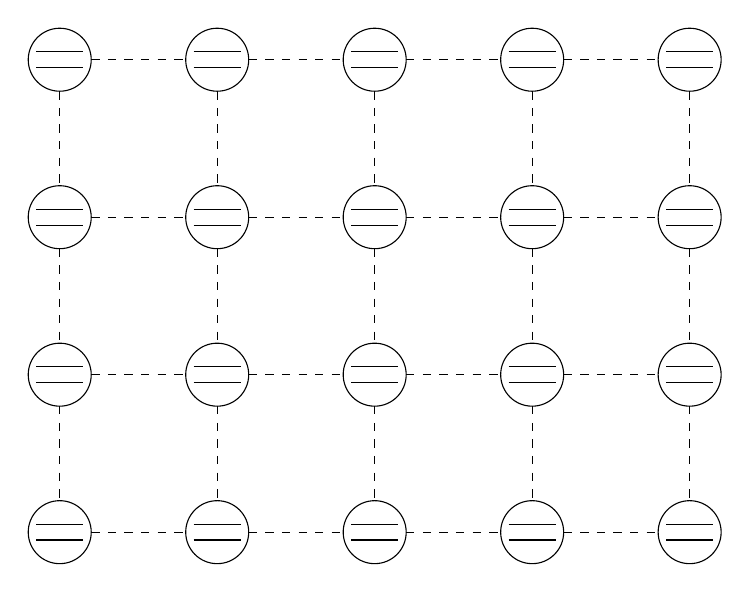
\begin{tikzpicture}
    \def\radius{0.4} % radius of the circles
    \def\dist{2} % distance between the centers of the circles
    \def\lineLength{0.6} % length of the horizontal lines inside the circles
    \def\lineOffset{0.1}

    \foreach \i in {1,2,3,4} {
        \foreach \j in {1,2,3,4,5} {
            \draw (\j*\dist, -\i*\dist) circle (\radius);
            \draw (\j*\dist - \lineLength/2, -\i*\dist + \lineOffset) -- (\j*\dist + \lineLength/2, -\i*\dist + \lineOffset);
            \draw (\j*\dist - \lineLength/2, -\i*\dist - \lineOffset) -- (\j*\dist + \lineLength/2, -\i*\dist - \lineOffset);
        }
    }

    \foreach \i in {1,2,3,4} {
        \foreach \j in {1,2,3,4} {
            \draw[dashed] (\j*\dist + \radius, -\i*\dist) -- (\j*\dist + \dist - \radius, -\i*\dist);
        }
    }
    \foreach \i in {1,2,3} {
    \foreach \j in {1,2,3,4,5} {
        \draw[dashed] (\j*\dist, -\i*\dist - \radius) -- (\j*\dist, -\i*\dist - \dist + \radius);
    }
}

\end{tikzpicture}
\caption{A grid of $5 \times 4$ qubits.}
\label{fig:quantum_grid}
\end{figure}



\subsection{Superconducting Qubits}

Superconducting qubits are one of the many different realization of a quantum computer.\\
In this section I will briefly discuss how it is possible to obtain a two-level system starting from a superconducting circuit.

\paragraph*{LC circuit as an harmonic oscillator}

An LC circuit (figure~\ref{fig:lc_circuit}) is an electric circuit with a capacitor (with capacity C) and an inductor (with inductance L).
By indicating with V the voltage applied to the circuit and with I the current flowing in the circuit, the energy stored in the capacitor and
inductor will be:

\begin{align}
    E_C = \frac{1}{2}CV^2 = \frac{Q^2}{2C}
    \qquad
    E_L = \frac{1}{2}LI^2 = \frac{\phi^2}{2L}
\end{align}

Therefore the energy of the LC circuit will be:

\begin{equation}
    H_{LC} = \frac{Q^2}{2C} + \frac{\phi^2}{2L} = \frac{Q^2}{2C} + \frac{1}{2}C \omega_0^2 \phi^2 
\end{equation}

with $\omega_0 = 1 / \sqrt{LC}$.\\
This is the hamiltonian of an harmonic oscillator with mass C, momentum Q, position $\phi$ and frequency $\omega_0$, hence we can easily quantize
this system by promoting Q and $\phi$ to quantum operators:

\begin{align}
    \hat{Q} = i\sqrt{\frac{\hbar}{2 Z_0}}(\hat{a}^{\dagger} - \hat{a})
    \qquad
    \hat{\phi} = \sqrt{\frac{\hbar Z_0}{2}}(\hat{a}^{\dagger} + \hat{a})
\end{align}

where $Z_0= \sqrt{L / C}$ is the impedance.\\
$\hat{Q}$ and $\hat{\phi}$ obey to the canonical commutation relation:

\begin{equation}
    [\hat{Q}, \hat{\phi}] = i \hbar
\end{equation}

Therefore the hamiltonian for the quantized system is:

\begin{equation}
    H = \hbar \omega_0 (\hat{a}^{\dagger} \hat{a} + \frac{1}{2})
\end{equation}


A harmonic oscillator has infinitely many evenly spaced energy levels, making it unsuitable for quantum computation because it is impossible to 
isolate just two specific energy levels to represent a qubit.\\

\begin{figure}[ht]
    \centering
    \begin{tikzpicture}[scale=0.8] % Scale the circuit to make it smaller
        \draw
        % Draw the voltage source with two parallel lines
        (0,0) to[V, v={$V$}, invert] (0,4)
        
        % Draw the inductor L
        to[L, l={$L$}] (4,4)
        
        % Draw the capacitor C
        to[C, l={$C$}] (4,0)
        
        % Connect the circuit
        -- (0,0);
    \end{tikzpicture}
    \caption{An LC circuit with a voltage source ($V$), an inductor ($L$), and a capacitor ($C$) connected in series.}
    \label{fig:lc_circuit}
\end{figure}

\paragraph*{Josephson junction and SQUID}

To address the issue of isolating two specific energy levels to represent a qubit, it is necessary to introduce non-linearities that modify the energy spacing between levels, thus allowing us to select only two
levels that will be the qubit used for the computation.\\
These non-linearities can be introduced by a Josephson junction, which consists of two superconductors 
connected via a tunnelling barrier.
The classical hamiltonian of the Josephson juction is\footnote[1]{I have omitted the steps for deriving the Hamiltonian. 
Essentially, these steps involve transforming the Schrödinger equations for the superconductors in a Josephson junction into 
the Josephson equations. By solving these equations, one can easily determine the capacitance and inductance energy of the junction.}:

\begin{equation}
    H_J = \frac{Q^2}{2 C_J} - E_J cos(\psi) = 4 E_c N^2 - E_J cos(\phi)
\end{equation}

where $C_J$ is the capacitance of the junction, $E_J = (\phi_0 I_c) / (2 \pi)$\footnote[2]{$\phi_0$ = h / 2e and $I_c$ is the critical current of 
the junction.}, $\phi$ is the phase difference between the phases of the two superconductors of the junction, $E_c = e^2 / (2C_J)$, $N = N_1 - N_2$ 
where $N_1$ and $N_2$ represent the numbers of Cooper pairs present at each side of the junction.\\
Instead of considering only one Josephson junction we can consider a circuit with two junctions connected in parallel, which commonly referred to as SQUID 
(Superconducting QUantum Interference Device) device.
If the circuit has a voltage of $V_g$ the hamiltonian of the circuit shown in picture:

\begin{equation}
    H = 4 E_c (N - N_g)^2 - E_J cos(\phi)
\end{equation}

where the voltage $V_g$ has shifted N by $N_g = C_g V_g / (2e)$ and:

\begin{equation}
    E_J = \frac{e^2}{2(C_g + C_J)}
\end{equation}

The quantization of the hamiltonian just requires to promote N and $\phi$ to quantum operators:

\begin{equation}
    \hat{H} = 4 E_c (\hat{N} - N_g)^2 - E_J cos(\hat{\phi})
\label{eq:superconducting}
\end{equation}

where $\hat{N} \in (- \infty, + \infty)$ is the excess of Cooper pairs.
$\hat{N}$ and $\hat{\psi}$ satisfy the canonical commutation relation:

\begin{equation}
    [\hat{\phi}, \hat{N}] = i \hbar
\end{equation}

The hamiltonian of a superconducting qubit (equation~\ref{eq:superconducting}) has two possibles
regimes, where we can define a two level system which can be used as a qubit: the \textit{charge regime} ($E_c \gg E_J$) and 
the \textit{transmon regime} ($E_c \ll E_J$). 

\begin{figure}[ht]
    \centering
    \begin{tikzpicture}[scale=0.8] % Scale the circuit to make it smaller
        
        % Draw the ground
        \begin{scope}[transform canvas={rotate=-90}]
        \draw (0,0) node[ground, scale=2] {};
        \end{scope}
        
        % Draw the voltage source
        \draw (0,0) to[V, v={$V$}] (0,3);
        
        % Draw the capacitor
        \draw (0,3) to[C, l={$C_g$}] (3,3);
                
        % Draw the custom SQUID symbol
        \draw (3,0) to [squid, l^=$J_1$] (3,3) 
         (3,0) to [squid, l_=$J_2$] (3,3); 
        
        % Draw the reservoir
        \draw (1.8, 0) rectangle (4.2, -1);
        \node at (3, -0.5) {Reservoir}; % Text inside the box

    \end{tikzpicture}
    \caption{Circuit diagram including an electric ground, a voltage source ($V$), a capacitor ($C$), a SQUID device, and a reservoir.}
    \label{fig:circuit}

\end{figure}








